\documentclass[russian,a4paper,12pt]{scrartcl}
\usepackage{babel}
\usepackage[utf8]{inputenc}
\usepackage[left=3cm,right=1cm,top=1cm,bottom=1cm]{geometry}
\usepackage{misccorr}
\usepackage{amsmath}
\usepackage{minted}
\usepackage{graphicx}
\usepackage{xcolor}
\usepackage{hyperref}
 % Цвета для гиперссылок
\definecolor{linkcolor}{HTML}{799B03} % цвет ссылок
\definecolor{urlcolor}{HTML}{799B03} % цвет гиперссылок
\hypersetup{pdfstartview=FitH,  linkcolor=blue,urlcolor=blue, colorlinks=true}

\begin{document}
	\begin{center}
	
		\large{МИНИСТЕРСТВО ОБРАЗОВАНИЯ И НАУКИ\\ РОССИЙСКОЙ ВЕДЕРАЦИИ} \par
		\bf\MakeUppercase{федеральное государственное автономное образовательное учреждение высшего образования} \par
		\textit{<<Санкт-Петербургский Государственный университет 
		Аэрокосмического Приборостроения>>} \par
	
	\vspace{10mm}
		
		\MakeUppercase{Кафедра №14} \par 
		
	\vspace{20mm}
	\begin{flushleft}
		{ОТЧЕТ}\par
		{ЗАЩИЩЕН С ОЦЕНКОЙ}\par
		{ПРЕПОДАВАТЕЛЬ}\par
	\end{flushleft}
	\begin{flushleft}
			\[
			\underset{\text{должность}}{\underline{\hspace{1cm}\text{\strut асс.}\hspace{1cm}}}
			\quad\underset{\text{подпись, дата}}{\underline{\strut \hspace{4cm}}}
			\quad\underset{\text{инициалы, фамилия}}{\underline{\hspace{1cm}\text{\strut П.С. Санкин}\hspace{1cm}}}
			\]
	\end{flushleft}
	\vspace{10mm}

		 \textbf{ОТЧЕТ О ЛАБОРАТОРНОЙ РАБОТЕ №2}\par{Статистическое распределение элементов цифрового изображения}\par{По курсу: <<Основы мультимедия технологий>>.} \par
		
	\vspace{40mm}

	\begin{flushleft}
		{РАБОТУ ВЫПОЛНИЛ}\par
		\begin{flushleft}
			СТУДЕНТ ГРУППЫ 
			\underline{\strut 1441} 
			\quad\underset{\text{подпись, дата}}{\underline{\strut \hspace{3cm}}}\quad
			\underset{\text{инициалы, фамилия}}{\underline{\text{\strut А.А. Протасов}}}
		\end{flushleft}
	\end{flushleft}

	\vspace{50mm}
	
		{Санкт-Петербург\\ 2016}
	\thispagestyle{empty}
	\newpage
	
	\end{center}

	\begin{flushleft}
		\section{Цель работы}
			Hеализовать программу выполняющую построение гистограммы для растрового изображения.
		\section{Постановка задачи}
			Для графических файлов написать программу выполняющую построение гистограммы для растрового изображения. Программа должна иметь элементы управления отдельными цветовыми каналами изображения согласно заданию. Гистограмма должна быть построена как для исходного, так и для преобразованного изображения.\\
			Графические файлы для проверки изображений создать самостоятельно.
		\section{Задание}
			Управление яркостью для всех каналов.
		\section{Краткие теоритические сведения}
			Гистограмма — способ графического представления табличных данных.\\
			Количественные соотношения некоторого показателя представлены в виде прямоугольников, площади которых пропорциональны. Чаще всего для удобства восприятия ширину прямоугольников берут одинаковую, при этом их высота определяет соотношения отображаемого параметра.//
			Гистограмма в фотографии — это график статистического распределения элементов цифрового изображения с различной яркостью, в котором по горизонтальной оси представлена яркость, а по вертикали — относительное число пикселов с конкретным значением яркости.
		\section{Описание метода реализации}
			Программа была написана в среде для разработки Qt с использованием библиотеки компьютерного зрения OpenCV.\\
			Для открытия изображения и разделения цветовой палитры на разные каналы была использованиа библиотека OpenCV. Так-же из библиотеки OpenCV был использован шаблон sturate\_cast для преобразовния целого значения(исходное значение пикселя плюс значение на которое мы увеличиваем яркось) в понятное для типа Mat 8-битное значение.
	\end{flushleft}
	\newpage
	\section{Листинги}
	\usemintedstyle{autumn}
	\subsection{\text{Тело основной функции}}
		\inputminted[
			frame=lines,
			framesep=2mm,
			baselinestretch=1.2,
			fontsize=\footnotesize,
			linenos
			]{cpp}{main.cpp}
	\subsection{\text{Заголовок класса главного окна}}
		\inputminted[
			frame=lines,
			framesep=2mm,
			baselinestretch=1.2,
			fontsize=\footnotesize,
			linenos
			]{cpp}{mainwindow.h}
	\subsection{\text{Описание методов класса главного окна}}
		\inputminted[
			frame=lines,
			framesep=2mm,
			baselinestretch=1.2,
			fontsize=\footnotesize,
			linenos
			]{cpp}{mainwindow.cpp}
	\subsection{\text{Описание формы главного окна}}
		\inputminted[
			frame=lines,
			framesep=2mm,
			baselinestretch=1.2,
			fontsize=\footnotesize,
			linenos
			]{xml}{mainwindow.ui}
	\section{Примеры работы программы}
		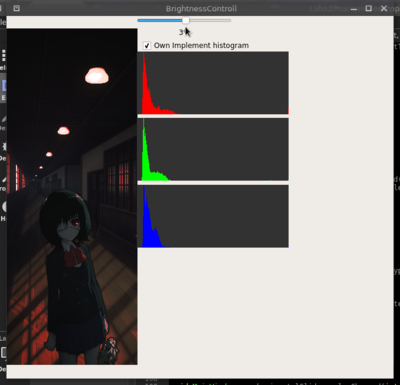
\includegraphics{screen3}\\
		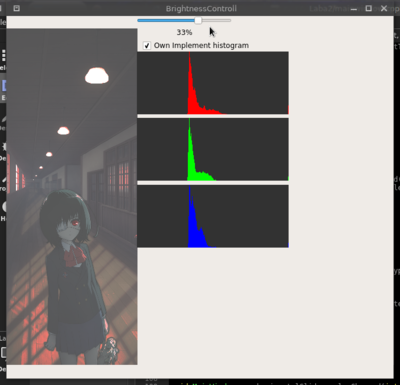
\includegraphics{screen4}
	\newpage
	\begin{thebibliography}{9}
		\bibitem{Shlee-2015}Шлее М. Qt 5.3. Профессиональное программирование на C++ \newblock --- Санкт-Петербург:
		Изд.  БХВ-Петербург, 2015. 928~с.
		\bibitem{Qt-reference} \href{http://doc.qt.io/qt-5/reference-overview.html}{\underline{http://doc.qt.io/qt-5/reference-overview.html}}
		\bibitem{Guide}Методические указания по курсу: ОСНОВЫ МУЛЬТИМЕДИАТЕХНОЛОГИЙ
	\end{thebibliography}
\end{document}